\documentclass[1p]{elsarticle_modified}
%\bibliographystyle{elsarticle-num}

%\usepackage[colorlinks]{hyperref}
%\usepackage{abbrmath_seonhwa} %\Abb, \Ascr, \Acal ,\Abf, \Afrak
\usepackage{amsfonts}
\usepackage{amssymb}
\usepackage{amsmath}
\usepackage{amsthm}
\usepackage{scalefnt}
\usepackage{amsbsy}
\usepackage{kotex}
\usepackage{caption}
\usepackage{subfig}
\usepackage{color}
\usepackage{graphicx}
\usepackage{xcolor} %% white, black, red, green, blue, cyan, magenta, yellow
\usepackage{float}
\usepackage{setspace}
\usepackage{hyperref}

\usepackage{tikz}
\usetikzlibrary{arrows}

\usepackage{multirow}
\usepackage{array} % fixed length table
\usepackage{hhline}

%%%%%%%%%%%%%%%%%%%%%
\makeatletter
\renewcommand*\env@matrix[1][\arraystretch]{%
	\edef\arraystretch{#1}%
	\hskip -\arraycolsep
	\let\@ifnextchar\new@ifnextchar
	\array{*\c@MaxMatrixCols c}}
\makeatother %https://tex.stackexchange.com/questions/14071/how-can-i-increase-the-line-spacing-in-a-matrix
%%%%%%%%%%%%%%%

\usepackage[normalem]{ulem}

\newcommand{\msout}[1]{\ifmmode\text{\sout{\ensuremath{#1}}}\else\sout{#1}\fi}
%SOURCE: \msout is \stkout macro in https://tex.stackexchange.com/questions/20609/strikeout-in-math-mode

\newcommand{\cancel}[1]{
	\ifmmode
	{\color{red}\msout{#1}}
	\else
	{\color{red}\sout{#1}}
	\fi
}

\newcommand{\add}[1]{
	{\color{blue}\uwave{#1}}
}

\newcommand{\replace}[2]{
	\ifmmode
	{\color{red}\msout{#1}}{\color{blue}\uwave{#2}}
	\else
	{\color{red}\sout{#1}}{\color{blue}\uwave{#2}}
	\fi
}

\newcommand{\Sol}{\mathcal{S}} %segment
\newcommand{\D}{D} %diagram
\newcommand{\A}{\mathcal{A}} %arc


%%%%%%%%%%%%%%%%%%%%%%%%%%%%%5 test

\def\sl{\operatorname{\textup{SL}}(2,\Cbb)}
\def\psl{\operatorname{\textup{PSL}}(2,\Cbb)}
\def\quan{\mkern 1mu \triangleright \mkern 1mu}

\theoremstyle{definition}
\newtheorem{thm}{Theorem}[section]
\newtheorem{prop}[thm]{Proposition}
\newtheorem{lem}[thm]{Lemma}
\newtheorem{ques}[thm]{Question}
\newtheorem{cor}[thm]{Corollary}
\newtheorem{defn}[thm]{Definition}
\newtheorem{exam}[thm]{Example}
\newtheorem{rmk}[thm]{Remark}
\newtheorem{alg}[thm]{Algorithm}

\newcommand{\I}{\sqrt{-1}}
\begin{document}

%\begin{frontmatter}
%
%\title{Boundary parabolic representations of knots up to 8 crossings}
%
%%% Group authors per affiliation:
%\author{Yunhi Cho} 
%\address{Department of Mathematics, University of Seoul, Seoul, Korea}
%\ead{yhcho@uos.ac.kr}
%
%
%\author{Seonhwa Kim} %\fnref{s_kim}}
%\address{Center for Geometry and Physics, Institute for Basic Science, Pohang, 37673, Korea}
%\ead{ryeona17@ibs.re.kr}
%
%\author{Hyuk Kim}
%\address{Department of Mathematical Sciences, Seoul National University, Seoul 08826, Korea}
%\ead{hyukkim@snu.ac.kr}
%
%\author{Seokbeom Yoon}
%\address{Department of Mathematical Sciences, Seoul National University, Seoul, 08826,  Korea}
%\ead{sbyoon15@snu.ac.kr}
%
%\begin{abstract}
%We find all boundary parabolic representation of knots up to 8 crossings.
%
%\end{abstract}
%\begin{keyword}
%    \MSC[2010] 57M25 
%\end{keyword}
%
%\end{frontmatter}

%\linenumbers
%\tableofcontents
%
\newcommand\colored[1]{\textcolor{white}{\rule[-0.35ex]{0.8em}{1.4ex}}\kern-0.8em\color{red} #1}%
%\newcommand\colored[1]{\textcolor{white}{ #1}\kern-2.17ex	\textcolor{white}{ #1}\kern-1.81ex	\textcolor{white}{ #1}\kern-2.15ex\color{red}#1	}

{\Large $\underline{12a_{1137}~(K12a_{1137})}$}

\setlength{\tabcolsep}{10pt}
\renewcommand{\arraystretch}{1.6}
\vspace{1cm}\begin{tabular}{m{100pt}>{\centering\arraybackslash}m{274pt}}
\multirow{5}{120pt}{
	\centering
	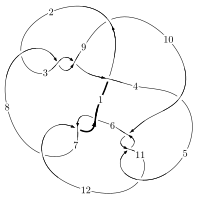
\includegraphics[width=112pt]{../../../GIT/diagram.site/Diagrams/png/1938_12a_1137.png}\\
\ \ \ A knot diagram\footnotemark}&
\allowdisplaybreaks
\textbf{Linearized knot diagam} \\
\cline{2-2}
 &
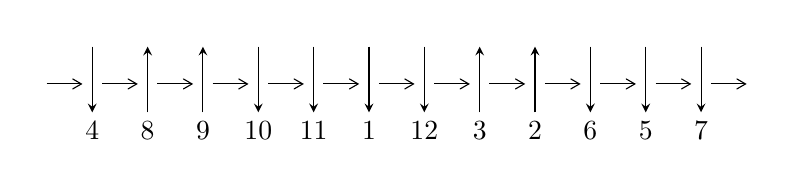
\begin{tikzpicture}[x=20pt, y=17pt]
	% nodes
	\node (C0) at (0, 0) {};
	\node (C1) at (1, 0) {};
	\node (C1U) at (1, +1) {};
	\node (C1D) at (1, -1) {4};

	\node (C2) at (2, 0) {};
	\node (C2U) at (2, +1) {};
	\node (C2D) at (2, -1) {8};

	\node (C3) at (3, 0) {};
	\node (C3U) at (3, +1) {};
	\node (C3D) at (3, -1) {9};

	\node (C4) at (4, 0) {};
	\node (C4U) at (4, +1) {};
	\node (C4D) at (4, -1) {10};

	\node (C5) at (5, 0) {};
	\node (C5U) at (5, +1) {};
	\node (C5D) at (5, -1) {11};

	\node (C6) at (6, 0) {};
	\node (C6U) at (6, +1) {};
	\node (C6D) at (6, -1) {1};

	\node (C7) at (7, 0) {};
	\node (C7U) at (7, +1) {};
	\node (C7D) at (7, -1) {12};

	\node (C8) at (8, 0) {};
	\node (C8U) at (8, +1) {};
	\node (C8D) at (8, -1) {3};

	\node (C9) at (9, 0) {};
	\node (C9U) at (9, +1) {};
	\node (C9D) at (9, -1) {2};

	\node (C10) at (10, 0) {};
	\node (C10U) at (10, +1) {};
	\node (C10D) at (10, -1) {6};

	\node (C11) at (11, 0) {};
	\node (C11U) at (11, +1) {};
	\node (C11D) at (11, -1) {5};

	\node (C12) at (12, 0) {};
	\node (C12U) at (12, +1) {};
	\node (C12D) at (12, -1) {7};
	\node (C13) at (13, 0) {};

	% arrows
	\draw[->,>={angle 60}]
	(C0) edge (C1) (C1) edge (C2) (C2) edge (C3) (C3) edge (C4) (C4) edge (C5) (C5) edge (C6) (C6) edge (C7) (C7) edge (C8) (C8) edge (C9) (C9) edge (C10) (C10) edge (C11) (C11) edge (C12) (C12) edge (C13) ;	\draw[->,>=stealth]
	(C1U) edge (C1D) (C2D) edge (C2U) (C3D) edge (C3U) (C4U) edge (C4D) (C5U) edge (C5D) (C6U) edge (C6D) (C7U) edge (C7D) (C8D) edge (C8U) (C9D) edge (C9U) (C10U) edge (C10D) (C11U) edge (C11D) (C12U) edge (C12D) ;
	\end{tikzpicture} \\
\hhline{~~} \\& 
\textbf{Solving Sequence} \\ \cline{2-2} 
 &
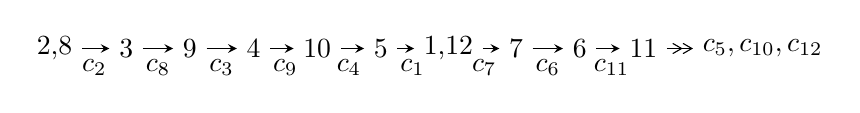
\begin{tikzpicture}[x=23pt, y=7pt]
	% node
	\node (A0) at (-1/8, 0) {2,8};
	\node (A1) at (1, 0) {3};
	\node (A2) at (2, 0) {9};
	\node (A3) at (3, 0) {4};
	\node (A4) at (4, 0) {10};
	\node (A5) at (5, 0) {5};
	\node (A6) at (97/16, 0) {1,12};
	\node (A7) at (57/8, 0) {7};
	\node (A8) at (65/8, 0) {6};
	\node (A9) at (73/8, 0) {11};
	\node (C1) at (1/2, -1) {$c_{2}$};
	\node (C2) at (3/2, -1) {$c_{8}$};
	\node (C3) at (5/2, -1) {$c_{3}$};
	\node (C4) at (7/2, -1) {$c_{9}$};
	\node (C5) at (9/2, -1) {$c_{4}$};
	\node (C6) at (11/2, -1) {$c_{1}$};
	\node (C7) at (53/8, -1) {$c_{7}$};
	\node (C8) at (61/8, -1) {$c_{6}$};
	\node (C9) at (69/8, -1) {$c_{11}$};
	\node (A10) at (11, 0) {$c_{5},c_{10},c_{12}$};

	% edge
	\draw[->,>=stealth]	
	(A0) edge (A1) (A1) edge (A2) (A2) edge (A3) (A3) edge (A4) (A4) edge (A5) (A5) edge (A6) (A6) edge (A7) (A7) edge (A8) (A8) edge (A9) ;
	\draw[->>,>={angle 60}]	
	(A9) edge (A10);
\end{tikzpicture} \\ 

\end{tabular} \\

\footnotetext{
The image of knot diagram is generated by the software ``\textbf{Draw programme}" developed by Andrew Bartholomew(\url{http://www.layer8.co.uk/maths/draw/index.htm\#Running-draw}), where we modified some parts for our purpose(\url{https://github.com/CATsTAILs/LinksPainter}).
}\phantom \\ \newline 
\centering \textbf{Ideals for irreducible components\footnotemark of $X_{\text{par}}$} 
 
\begin{align*}
I^u_{1}&=\langle 
3 u^{29}-5 u^{28}+\cdots+b-3,\;- u^{29}+u^{28}+\cdots+2 a-1,\;u^{30}-3 u^{29}+\cdots+3 u+2\rangle \\
I^u_{2}&=\langle 
u^{22} a- u^{22}+\cdots+b-1,\;u^{22}-11 u^{20}+\cdots+a^2+u,\;u^{23}+u^{22}+\cdots-2 u^3+1\rangle \\
I^u_{3}&=\langle 
u^3+b- u-1,\;- u^4+2 u^2+a-1,\;u^6-3 u^4+2 u^2+1\rangle \\
\\
\end{align*}
\raggedright * 3 irreducible components of $\dim_{\mathbb{C}}=0$, with total 82 representations.\\
\footnotetext{All coefficients of polynomials are rational numbers. But the coefficients are sometimes approximated in decimal forms when there is not enough margin.}
\newpage
\renewcommand{\arraystretch}{1}
\centering \section*{I. $I^u_{1}= \langle 3 u^{29}-5 u^{28}+\cdots+b-3,\;- u^{29}+u^{28}+\cdots+2 a-1,\;u^{30}-3 u^{29}+\cdots+3 u+2 \rangle$}
\flushleft \textbf{(i) Arc colorings}\\
\begin{tabular}{m{7pt} m{180pt} m{7pt} m{180pt} }
\flushright $a_{2}=$&$\begin{pmatrix}1\\0\end{pmatrix}$ \\
\flushright $a_{8}=$&$\begin{pmatrix}0\\u\end{pmatrix}$ \\
\flushright $a_{3}=$&$\begin{pmatrix}1\\- u^2\end{pmatrix}$ \\
\flushright $a_{9}=$&$\begin{pmatrix}u\\- u^3+u\end{pmatrix}$ \\
\flushright $a_{4}=$&$\begin{pmatrix}- u^2+1\\u^4-2 u^2\end{pmatrix}$ \\
\flushright $a_{10}=$&$\begin{pmatrix}- u^3+2 u\\- u^3+u\end{pmatrix}$ \\
\flushright $a_{5}=$&$\begin{pmatrix}- u^{10}+5 u^8-8 u^6+3 u^4+u^2+1\\- u^{10}+4 u^8-5 u^6+2 u^4- u^2\end{pmatrix}$ \\
\flushright $a_{1}=$&$\begin{pmatrix}u^6-3 u^4+2 u^2+1\\- u^8+4 u^6-4 u^4\end{pmatrix}$ \\
\flushright $a_{12}=$&$\begin{pmatrix}\frac{1}{2} u^{29}-\frac{1}{2} u^{28}+\cdots- u+\frac{1}{2}\\-3 u^{29}+5 u^{28}+\cdots+6 u+3\end{pmatrix}$ \\
\flushright $a_{7}=$&$\begin{pmatrix}\frac{1}{2} u^{29}-\frac{1}{2} u^{28}+\cdots-3 u-\frac{3}{2}\\2 u^{29}-3 u^{28}+\cdots-6 u-3\end{pmatrix}$ \\
\flushright $a_{6}=$&$\begin{pmatrix}\frac{3}{2} u^{29}-\frac{3}{2} u^{28}+\cdots-9 u-\frac{9}{2}\\5 u^{29}-7 u^{28}+\cdots-16 u-7\end{pmatrix}$ \\
\flushright $a_{11}=$&$\begin{pmatrix}\frac{1}{2} u^{29}-\frac{1}{2} u^{28}+\cdots-2 u^2-\frac{1}{2}\\- u^{29}+2 u^{28}+\cdots+3 u+1\end{pmatrix}$\\&\end{tabular}
\flushleft \textbf{(ii) Obstruction class $= -1$}\\~\\
\flushleft \textbf{(iii) Cusp Shapes $= 4 u^{29}-6 u^{28}-44 u^{27}+58 u^{26}+214 u^{25}-222 u^{24}-596 u^{23}+376 u^{22}+1006 u^{21}-58 u^{20}-920 u^{19}-828 u^{18}+88 u^{17}+1268 u^{16}+752 u^{15}-520 u^{14}-658 u^{13}-320 u^{12}+76 u^{11}+234 u^{10}-14 u^9-2 u^8+148 u^7+92 u^6+38 u^5-30 u^4-80 u^3-44 u^2-24 u-18$}\\~\\
\newpage\renewcommand{\arraystretch}{1}
\flushleft \textbf{(iv) u-Polynomials at the component}\newline \\
\begin{tabular}{m{50pt}|m{274pt}}
Crossings & \hspace{64pt}u-Polynomials at each crossing \\
\hline $$\begin{aligned}c_{1}\end{aligned}$$&$\begin{aligned}
&u^{30}-7 u^{29}+\cdots-415 u+136
\end{aligned}$\\
\hline $$\begin{aligned}c_{2},c_{3},c_{8}\end{aligned}$$&$\begin{aligned}
&u^{30}-3 u^{29}+\cdots+3 u+2
\end{aligned}$\\
\hline $$\begin{aligned}c_{4}\end{aligned}$$&$\begin{aligned}
&u^{30}+3 u^{29}+\cdots+320 u+128
\end{aligned}$\\
\hline $$\begin{aligned}c_{5},c_{6},c_{7}\\c_{10},c_{11},c_{12}\end{aligned}$$&$\begin{aligned}
&u^{30}+16 u^{28}+\cdots+u+1
\end{aligned}$\\
\hline $$\begin{aligned}c_{9}\end{aligned}$$&$\begin{aligned}
&u^{30}+9 u^{29}+\cdots+93 u+6
\end{aligned}$\\
\hline
\end{tabular}\\~\\
\newpage\renewcommand{\arraystretch}{1}
\flushleft \textbf{(v) Riley Polynomials at the component}\newline \\
\begin{tabular}{m{50pt}|m{274pt}}
Crossings & \hspace{64pt}Riley Polynomials at each crossing \\
\hline $$\begin{aligned}c_{1}\end{aligned}$$&$\begin{aligned}
&y^{30}+5 y^{29}+\cdots+17087 y+18496
\end{aligned}$\\
\hline $$\begin{aligned}c_{2},c_{3},c_{8}\end{aligned}$$&$\begin{aligned}
&y^{30}-27 y^{29}+\cdots+15 y+4
\end{aligned}$\\
\hline $$\begin{aligned}c_{4}\end{aligned}$$&$\begin{aligned}
&y^{30}-5 y^{29}+\cdots+323584 y+16384
\end{aligned}$\\
\hline $$\begin{aligned}c_{5},c_{6},c_{7}\\c_{10},c_{11},c_{12}\end{aligned}$$&$\begin{aligned}
&y^{30}+32 y^{29}+\cdots+9 y+1
\end{aligned}$\\
\hline $$\begin{aligned}c_{9}\end{aligned}$$&$\begin{aligned}
&y^{30}+y^{29}+\cdots-2433 y+36
\end{aligned}$\\
\hline
\end{tabular}\\~\\
\newpage\flushleft \textbf{(vi) Complex Volumes and Cusp Shapes}
$$\begin{array}{c|c|c}  
\text{Solutions to }I^u_{1}& \I (\text{vol} + \sqrt{-1}CS) & \text{Cusp shape}\\
 \hline 
\begin{aligned}
u &= -0.930902\phantom{ +0.000000I} \\
a &= \phantom{-}0.756247\phantom{ +0.000000I} \\
b &= -1.08322\phantom{ +0.000000I}\end{aligned}
 & -1.46218\phantom{ +0.000000I} & -7.28610\phantom{ +0.000000I} \\ \hline\begin{aligned}
u &= -1.089660 + 0.308662 I \\
a &= \phantom{-}0.099048 - 1.205780 I \\
b &= \phantom{-}1.65581 + 0.20452 I\end{aligned}
 & \phantom{-}6.92010 - 7.02665 I & \phantom{-}2.40937 + 6.27539 I \\ \hline\begin{aligned}
u &= -1.089660 - 0.308662 I \\
a &= \phantom{-}0.099048 + 1.205780 I \\
b &= \phantom{-}1.65581 - 0.20452 I\end{aligned}
 & \phantom{-}6.92010 + 7.02665 I & \phantom{-}2.40937 - 6.27539 I \\ \hline\begin{aligned}
u &= -0.704410 + 0.436123 I \\
a &= -1.21026 + 1.24528 I \\
b &= \phantom{-}0.040668 - 0.499528 I\end{aligned}
 & \phantom{-}7.95280 + 7.12520 I & \phantom{-}2.76356 - 2.96102 I \\ \hline\begin{aligned}
u &= -0.704410 - 0.436123 I \\
a &= -1.21026 - 1.24528 I \\
b &= \phantom{-}0.040668 + 0.499528 I\end{aligned}
 & \phantom{-}7.95280 - 7.12520 I & \phantom{-}2.76356 + 2.96102 I \\ \hline\begin{aligned}
u &= -0.304786 + 0.743959 I \\
a &= -1.46293 + 1.06283 I \\
b &= -1.36076 + 1.49177 I\end{aligned}
 & \phantom{-}6.54937 - 11.30350 I & \phantom{-}0.19641 + 8.01251 I \\ \hline\begin{aligned}
u &= -0.304786 - 0.743959 I \\
a &= -1.46293 - 1.06283 I \\
b &= -1.36076 - 1.49177 I\end{aligned}
 & \phantom{-}6.54937 + 11.30350 I & \phantom{-}0.19641 - 8.01251 I \\ \hline\begin{aligned}
u &= -0.103486 + 0.765219 I \\
a &= \phantom{-}1.73841 + 0.04408 I \\
b &= \phantom{-}1.54138 + 0.39049 I\end{aligned}
 & \phantom{-}3.91072 + 3.07613 I & -0.68680 - 2.45527 I \\ \hline\begin{aligned}
u &= -0.103486 - 0.765219 I \\
a &= \phantom{-}1.73841 - 0.04408 I \\
b &= \phantom{-}1.54138 - 0.39049 I\end{aligned}
 & \phantom{-}3.91072 - 3.07613 I & -0.68680 + 2.45527 I \\ \hline\begin{aligned}
u &= \phantom{-}0.463501 + 0.614076 I \\
a &= -1.51718 - 1.19039 I \\
b &= -0.727847 - 0.567986 I\end{aligned}
 & \phantom{-}11.82910 + 2.06121 I & \phantom{-}4.42340 - 3.33690 I\\
 \hline 
 \end{array}$$\newpage$$\begin{array}{c|c|c}  
\text{Solutions to }I^u_{1}& \I (\text{vol} + \sqrt{-1}CS) & \text{Cusp shape}\\
 \hline 
\begin{aligned}
u &= \phantom{-}0.463501 - 0.614076 I \\
a &= -1.51718 + 1.19039 I \\
b &= -0.727847 + 0.567986 I\end{aligned}
 & \phantom{-}11.82910 - 2.06121 I & \phantom{-}4.42340 + 3.33690 I \\ \hline\begin{aligned}
u &= -0.229240 + 0.685867 I \\
a &= -0.139869 - 1.010570 I \\
b &= -0.032234 - 1.383400 I\end{aligned}
 & -3.39097 - 3.33199 I & -9.55544 + 5.59326 I \\ \hline\begin{aligned}
u &= -0.229240 - 0.685867 I \\
a &= -0.139869 + 1.010570 I \\
b &= -0.032234 + 1.383400 I\end{aligned}
 & -3.39097 + 3.33199 I & -9.55544 - 5.59326 I \\ \hline\begin{aligned}
u &= -0.680122\phantom{ +0.000000I} \\
a &= \phantom{-}0.965666\phantom{ +0.000000I} \\
b &= -0.665414\phantom{ +0.000000I}\end{aligned}
 & -1.48461\phantom{ +0.000000I} & -6.75330\phantom{ +0.000000I} \\ \hline\begin{aligned}
u &= \phantom{-}1.307540 + 0.319637 I \\
a &= \phantom{-}0.353413 + 0.920897 I \\
b &= \phantom{-}1.132810 - 0.600648 I\end{aligned}
 & \phantom{-}8.31617 + 0.83782 I & \phantom{-}4.44779 + 0.17762 I \\ \hline\begin{aligned}
u &= \phantom{-}1.307540 - 0.319637 I \\
a &= \phantom{-}0.353413 - 0.920897 I \\
b &= \phantom{-}1.132810 + 0.600648 I\end{aligned}
 & \phantom{-}8.31617 - 0.83782 I & \phantom{-}4.44779 - 0.17762 I \\ \hline\begin{aligned}
u &= \phantom{-}1.352520 + 0.135874 I \\
a &= \phantom{-}0.381110 + 0.172911 I \\
b &= -0.383620 + 0.193018 I\end{aligned}
 & \phantom{-}3.75541 + 0.77985 I & -2.27872 + 2.76052 I \\ \hline\begin{aligned}
u &= \phantom{-}1.352520 - 0.135874 I \\
a &= \phantom{-}0.381110 - 0.172911 I \\
b &= -0.383620 - 0.193018 I\end{aligned}
 & \phantom{-}3.75541 - 0.77985 I & -2.27872 - 2.76052 I \\ \hline\begin{aligned}
u &= -1.350210 + 0.200800 I \\
a &= -0.056070 - 0.361065 I \\
b &= \phantom{-}0.555528 - 0.782092 I\end{aligned}
 & \phantom{-}4.51414 - 3.42768 I & -0.15581 + 5.80126 I \\ \hline\begin{aligned}
u &= -1.350210 - 0.200800 I \\
a &= -0.056070 + 0.361065 I \\
b &= \phantom{-}0.555528 + 0.782092 I\end{aligned}
 & \phantom{-}4.51414 + 3.42768 I & -0.15581 - 5.80126 I\\
 \hline 
 \end{array}$$\newpage$$\begin{array}{c|c|c}  
\text{Solutions to }I^u_{1}& \I (\text{vol} + \sqrt{-1}CS) & \text{Cusp shape}\\
 \hline 
\begin{aligned}
u &= \phantom{-}1.38985 + 0.27006 I \\
a &= -0.489440 + 0.230842 I \\
b &= \phantom{-}1.07204 + 1.56270 I\end{aligned}
 & \phantom{-}1.76191 + 6.80641 I & -4.17068 - 6.44926 I \\ \hline\begin{aligned}
u &= \phantom{-}1.38985 - 0.27006 I \\
a &= -0.489440 - 0.230842 I \\
b &= \phantom{-}1.07204 - 1.56270 I\end{aligned}
 & \phantom{-}1.76191 - 6.80641 I & -4.17068 + 6.44926 I \\ \hline\begin{aligned}
u &= \phantom{-}1.42853 + 0.29221 I \\
a &= \phantom{-}0.046116 - 1.008880 I \\
b &= -2.90289 - 1.59266 I\end{aligned}
 & \phantom{-}12.0906 + 15.0680 I & \phantom{-}4.25091 - 8.34423 I \\ \hline\begin{aligned}
u &= \phantom{-}1.42853 - 0.29221 I \\
a &= \phantom{-}0.046116 + 1.008880 I \\
b &= -2.90289 + 1.59266 I\end{aligned}
 & \phantom{-}12.0906 - 15.0680 I & \phantom{-}4.25091 + 8.34423 I \\ \hline\begin{aligned}
u &= \phantom{-}1.46604 + 0.09649 I \\
a &= -0.257035 - 0.974980 I \\
b &= \phantom{-}0.50288 - 1.41355 I\end{aligned}
 & \phantom{-}14.8637 - 5.5424 I & \phantom{-}6.83012 + 3.12730 I \\ \hline\begin{aligned}
u &= \phantom{-}1.46604 - 0.09649 I \\
a &= -0.257035 + 0.974980 I \\
b &= \phantom{-}0.50288 + 1.41355 I\end{aligned}
 & \phantom{-}14.8637 + 5.5424 I & \phantom{-}6.83012 - 3.12730 I \\ \hline\begin{aligned}
u &= -1.46325 + 0.21014 I \\
a &= -0.110662 + 1.025770 I \\
b &= -1.28614 + 1.87885 I\end{aligned}
 & \phantom{-}18.0378 - 5.0287 I & \phantom{-}7.86103 + 3.20489 I \\ \hline\begin{aligned}
u &= -1.46325 - 0.21014 I \\
a &= -0.110662 - 1.025770 I \\
b &= -1.28614 - 1.87885 I\end{aligned}
 & \phantom{-}18.0378 + 5.0287 I & \phantom{-}7.86103 - 3.20489 I \\ \hline\begin{aligned}
u &= \phantom{-}0.142590 + 0.468477 I \\
a &= \phantom{-}0.514389 + 0.535305 I \\
b &= \phantom{-}0.066704 + 0.337976 I\end{aligned}
 & -0.231238 + 0.878798 I & -5.31548 - 7.61341 I \\ \hline\begin{aligned}
u &= \phantom{-}0.142590 - 0.468477 I \\
a &= \phantom{-}0.514389 - 0.535305 I \\
b &= \phantom{-}0.066704 - 0.337976 I\end{aligned}
 & -0.231238 - 0.878798 I & -5.31548 + 7.61341 I\\
 \hline 
 \end{array}$$\newpage\newpage\renewcommand{\arraystretch}{1}
\centering \section*{II. $I^u_{2}= \langle u^{22} a- u^{22}+\cdots+b-1,\;u^{22}-11 u^{20}+\cdots+a^2+u,\;u^{23}+u^{22}+\cdots-2 u^3+1 \rangle$}
\flushleft \textbf{(i) Arc colorings}\\
\begin{tabular}{m{7pt} m{180pt} m{7pt} m{180pt} }
\flushright $a_{2}=$&$\begin{pmatrix}1\\0\end{pmatrix}$ \\
\flushright $a_{8}=$&$\begin{pmatrix}0\\u\end{pmatrix}$ \\
\flushright $a_{3}=$&$\begin{pmatrix}1\\- u^2\end{pmatrix}$ \\
\flushright $a_{9}=$&$\begin{pmatrix}u\\- u^3+u\end{pmatrix}$ \\
\flushright $a_{4}=$&$\begin{pmatrix}- u^2+1\\u^4-2 u^2\end{pmatrix}$ \\
\flushright $a_{10}=$&$\begin{pmatrix}- u^3+2 u\\- u^3+u\end{pmatrix}$ \\
\flushright $a_{5}=$&$\begin{pmatrix}- u^{10}+5 u^8-8 u^6+3 u^4+u^2+1\\- u^{10}+4 u^8-5 u^6+2 u^4- u^2\end{pmatrix}$ \\
\flushright $a_{1}=$&$\begin{pmatrix}u^6-3 u^4+2 u^2+1\\- u^8+4 u^6-4 u^4\end{pmatrix}$ \\
\flushright $a_{12}=$&$\begin{pmatrix}a\\- u^{22} a+u^{22}+\cdots- u+1\end{pmatrix}$ \\
\flushright $a_{7}=$&$\begin{pmatrix}u^{22}+u^{21}+\cdots- u^2+1\\- u^{22} a+u^{21}+\cdots- a+u\end{pmatrix}$ \\
\flushright $a_{6}=$&$\begin{pmatrix}u^{22}+u^{21}+\cdots+a u+1\\- u^{22} a+u^{21}+\cdots- a+u\end{pmatrix}$ \\
\flushright $a_{11}=$&$\begin{pmatrix}u^{17}-8 u^{15}+\cdots+a+1\\- u^{22} a+u^{22}+\cdots- u^2 a+1\end{pmatrix}$\\&\end{tabular}
\flushleft \textbf{(ii) Obstruction class $= -1$}\\~\\
\flushleft \textbf{(iii) Cusp Shapes $= -4 u^{20}+36 u^{18}-4 u^{17}-132 u^{16}+32 u^{15}+244 u^{14}-100 u^{13}-220 u^{12}+144 u^{11}+60 u^{10}-80 u^9+24 u^8+4 u^6-12 u^5-8 u^4+20 u^3-4 u^2-2$}\\~\\
\newpage\renewcommand{\arraystretch}{1}
\flushleft \textbf{(iv) u-Polynomials at the component}\newline \\
\begin{tabular}{m{50pt}|m{274pt}}
Crossings & \hspace{64pt}u-Polynomials at each crossing \\
\hline $$\begin{aligned}c_{1}\end{aligned}$$&$\begin{aligned}
&(u^{23}-5 u^{22}+\cdots+32 u-7)^{2}
\end{aligned}$\\
\hline $$\begin{aligned}c_{2},c_{3},c_{8}\end{aligned}$$&$\begin{aligned}
&(u^{23}+u^{22}+\cdots-2 u^3+1)^{2}
\end{aligned}$\\
\hline $$\begin{aligned}c_{4}\end{aligned}$$&$\begin{aligned}
&(u^{23}- u^{22}+\cdots-8 u+5)^{2}
\end{aligned}$\\
\hline $$\begin{aligned}c_{5},c_{6},c_{7}\\c_{10},c_{11},c_{12}\end{aligned}$$&$\begin{aligned}
&u^{46}- u^{45}+\cdots-18 u+5
\end{aligned}$\\
\hline $$\begin{aligned}c_{9}\end{aligned}$$&$\begin{aligned}
&(u^{23}-3 u^{22}+\cdots+4 u-1)^{2}
\end{aligned}$\\
\hline
\end{tabular}\\~\\
\newpage\renewcommand{\arraystretch}{1}
\flushleft \textbf{(v) Riley Polynomials at the component}\newline \\
\begin{tabular}{m{50pt}|m{274pt}}
Crossings & \hspace{64pt}Riley Polynomials at each crossing \\
\hline $$\begin{aligned}c_{1}\end{aligned}$$&$\begin{aligned}
&(y^{23}+7 y^{22}+\cdots-404 y-49)^{2}
\end{aligned}$\\
\hline $$\begin{aligned}c_{2},c_{3},c_{8}\end{aligned}$$&$\begin{aligned}
&(y^{23}-21 y^{22}+\cdots-6 y^2-1)^{2}
\end{aligned}$\\
\hline $$\begin{aligned}c_{4}\end{aligned}$$&$\begin{aligned}
&(y^{23}-5 y^{22}+\cdots+264 y-25)^{2}
\end{aligned}$\\
\hline $$\begin{aligned}c_{5},c_{6},c_{7}\\c_{10},c_{11},c_{12}\end{aligned}$$&$\begin{aligned}
&y^{46}+35 y^{45}+\cdots-264 y+25
\end{aligned}$\\
\hline $$\begin{aligned}c_{9}\end{aligned}$$&$\begin{aligned}
&(y^{23}- y^{22}+\cdots+4 y-1)^{2}
\end{aligned}$\\
\hline
\end{tabular}\\~\\
\newpage\flushleft \textbf{(vi) Complex Volumes and Cusp Shapes}
$$\begin{array}{c|c|c}  
\text{Solutions to }I^u_{2}& \I (\text{vol} + \sqrt{-1}CS) & \text{Cusp shape}\\
 \hline 
\begin{aligned}
u &= \phantom{-}1.070060 + 0.182203 I \\
a &= -0.070084 + 1.156430 I \\
b &= \phantom{-}1.59533 - 0.13562 I\end{aligned}
 & \phantom{-}2.26450 + 3.60580 I & -2.88555 - 4.48858 I \\ \hline\begin{aligned}
u &= \phantom{-}1.070060 + 0.182203 I \\
a &= \phantom{-}0.603866 - 0.224449 I \\
b &= -1.405470 - 0.026465 I\end{aligned}
 & \phantom{-}2.26450 + 3.60580 I & -2.88555 - 4.48858 I \\ \hline\begin{aligned}
u &= \phantom{-}1.070060 - 0.182203 I \\
a &= -0.070084 - 1.156430 I \\
b &= \phantom{-}1.59533 + 0.13562 I\end{aligned}
 & \phantom{-}2.26450 - 3.60580 I & -2.88555 + 4.48858 I \\ \hline\begin{aligned}
u &= \phantom{-}1.070060 - 0.182203 I \\
a &= \phantom{-}0.603866 + 0.224449 I \\
b &= -1.405470 + 0.026465 I\end{aligned}
 & \phantom{-}2.26450 - 3.60580 I & -2.88555 + 4.48858 I \\ \hline\begin{aligned}
u &= -1.15018\phantom{ +0.000000I} \\
a &= -0.261144 + 0.980051 I \\
b &= \phantom{-}1.95558 - 0.15361 I\end{aligned}
 & \phantom{-}5.24303\phantom{ +0.000000I} & \phantom{-}1.52610\phantom{ +0.000000I} \\ \hline\begin{aligned}
u &= -1.15018\phantom{ +0.000000I} \\
a &= -0.261144 - 0.980051 I \\
b &= \phantom{-}1.95558 + 0.15361 I\end{aligned}
 & \phantom{-}5.24303\phantom{ +0.000000I} & \phantom{-}1.52610\phantom{ +0.000000I} \\ \hline\begin{aligned}
u &= \phantom{-}0.285113 + 0.703745 I \\
a &= -0.120117 + 1.147110 I \\
b &= \phantom{-}0.22592 + 1.52660 I\end{aligned}
 & \phantom{-}1.28846 + 7.02777 I & -3.56401 - 7.34039 I \\ \hline\begin{aligned}
u &= \phantom{-}0.285113 + 0.703745 I \\
a &= -1.49794 - 1.02732 I \\
b &= -1.14402 - 1.60438 I\end{aligned}
 & \phantom{-}1.28846 + 7.02777 I & -3.56401 - 7.34039 I \\ \hline\begin{aligned}
u &= \phantom{-}0.285113 - 0.703745 I \\
a &= -0.120117 - 1.147110 I \\
b &= \phantom{-}0.22592 - 1.52660 I\end{aligned}
 & \phantom{-}1.28846 - 7.02777 I & -3.56401 + 7.34039 I \\ \hline\begin{aligned}
u &= \phantom{-}0.285113 - 0.703745 I \\
a &= -1.49794 + 1.02732 I \\
b &= -1.14402 + 1.60438 I\end{aligned}
 & \phantom{-}1.28846 - 7.02777 I & -3.56401 + 7.34039 I\\
 \hline 
 \end{array}$$\newpage$$\begin{array}{c|c|c}  
\text{Solutions to }I^u_{2}& \I (\text{vol} + \sqrt{-1}CS) & \text{Cusp shape}\\
 \hline 
\begin{aligned}
u &= \phantom{-}0.625021 + 0.336059 I \\
a &= \phantom{-}1.106610 - 0.179524 I \\
b &= -0.474160 - 0.683912 I\end{aligned}
 & \phantom{-}2.66992 - 3.26242 I & -0.80376 + 2.26815 I \\ \hline\begin{aligned}
u &= \phantom{-}0.625021 + 0.336059 I \\
a &= -1.18555 - 1.45591 I \\
b &= \phantom{-}0.343202 + 0.182577 I\end{aligned}
 & \phantom{-}2.66992 - 3.26242 I & -0.80376 + 2.26815 I \\ \hline\begin{aligned}
u &= \phantom{-}0.625021 - 0.336059 I \\
a &= \phantom{-}1.106610 + 0.179524 I \\
b &= -0.474160 + 0.683912 I\end{aligned}
 & \phantom{-}2.66992 + 3.26242 I & -0.80376 - 2.26815 I \\ \hline\begin{aligned}
u &= \phantom{-}0.625021 - 0.336059 I \\
a &= -1.18555 + 1.45591 I \\
b &= \phantom{-}0.343202 - 0.182577 I\end{aligned}
 & \phantom{-}2.66992 + 3.26242 I & -0.80376 - 2.26815 I \\ \hline\begin{aligned}
u &= -0.284234 + 0.630366 I \\
a &= \phantom{-}1.56548 + 0.06970 I \\
b &= \phantom{-}0.841978 + 0.781651 I\end{aligned}
 & \phantom{-}3.51028 - 2.29224 I & -0.17333 + 3.81893 I \\ \hline\begin{aligned}
u &= -0.284234 + 0.630366 I \\
a &= -1.60090 + 1.02304 I \\
b &= -0.68342 + 1.61231 I\end{aligned}
 & \phantom{-}3.51028 - 2.29224 I & -0.17333 + 3.81893 I \\ \hline\begin{aligned}
u &= -0.284234 - 0.630366 I \\
a &= \phantom{-}1.56548 - 0.06970 I \\
b &= \phantom{-}0.841978 - 0.781651 I\end{aligned}
 & \phantom{-}3.51028 + 2.29224 I & -0.17333 - 3.81893 I \\ \hline\begin{aligned}
u &= -0.284234 - 0.630366 I \\
a &= -1.60090 - 1.02304 I \\
b &= -0.68342 - 1.61231 I\end{aligned}
 & \phantom{-}3.51028 + 2.29224 I & -0.17333 - 3.81893 I \\ \hline\begin{aligned}
u &= \phantom{-}0.143415 + 0.670993 I \\
a &= -0.229021 + 0.764912 I \\
b &= -0.467867 + 1.159790 I\end{aligned}
 & -0.452611 - 0.303352 I & -7.41146 - 0.40480 I \\ \hline\begin{aligned}
u &= \phantom{-}0.143415 + 0.670993 I \\
a &= \phantom{-}1.68536 - 0.02244 I \\
b &= \phantom{-}1.182440 - 0.435170 I\end{aligned}
 & -0.452611 - 0.303352 I & -7.41146 - 0.40480 I\\
 \hline 
 \end{array}$$\newpage$$\begin{array}{c|c|c}  
\text{Solutions to }I^u_{2}& \I (\text{vol} + \sqrt{-1}CS) & \text{Cusp shape}\\
 \hline 
\begin{aligned}
u &= \phantom{-}0.143415 - 0.670993 I \\
a &= -0.229021 - 0.764912 I \\
b &= -0.467867 - 1.159790 I\end{aligned}
 & -0.452611 + 0.303352 I & -7.41146 + 0.40480 I \\ \hline\begin{aligned}
u &= \phantom{-}0.143415 - 0.670993 I \\
a &= \phantom{-}1.68536 + 0.02244 I \\
b &= \phantom{-}1.182440 + 0.435170 I\end{aligned}
 & -0.452611 + 0.303352 I & -7.41146 + 0.40480 I \\ \hline\begin{aligned}
u &= -1.347540 + 0.251864 I \\
a &= \phantom{-}0.317756 - 0.706992 I \\
b &= \phantom{-}0.719514 + 0.327199 I\end{aligned}
 & \phantom{-}4.24683 - 3.02476 I & -2.12213 + 2.21609 I \\ \hline\begin{aligned}
u &= -1.347540 + 0.251864 I \\
a &= -0.312944 - 0.116370 I \\
b &= \phantom{-}0.63476 - 1.57084 I\end{aligned}
 & \phantom{-}4.24683 - 3.02476 I & -2.12213 + 2.21609 I \\ \hline\begin{aligned}
u &= -1.347540 - 0.251864 I \\
a &= \phantom{-}0.317756 + 0.706992 I \\
b &= \phantom{-}0.719514 - 0.327199 I\end{aligned}
 & \phantom{-}4.24683 + 3.02476 I & -2.12213 - 2.21609 I \\ \hline\begin{aligned}
u &= -1.347540 - 0.251864 I \\
a &= -0.312944 + 0.116370 I \\
b &= \phantom{-}0.63476 + 1.57084 I\end{aligned}
 & \phantom{-}4.24683 + 3.02476 I & -2.12213 - 2.21609 I \\ \hline\begin{aligned}
u &= -0.405548 + 0.414027 I \\
a &= \phantom{-}0.39267 - 1.50726 I \\
b &= \phantom{-}0.861333 - 0.590644 I\end{aligned}
 & \phantom{-}4.30391 - 0.94673 I & \phantom{-}2.43633 + 4.33310 I \\ \hline\begin{aligned}
u &= -0.405548 + 0.414027 I \\
a &= -1.66459 + 1.46493 I \\
b &= \phantom{-}0.245747 + 0.579180 I\end{aligned}
 & \phantom{-}4.30391 - 0.94673 I & \phantom{-}2.43633 + 4.33310 I \\ \hline\begin{aligned}
u &= -0.405548 - 0.414027 I \\
a &= \phantom{-}0.39267 + 1.50726 I \\
b &= \phantom{-}0.861333 + 0.590644 I\end{aligned}
 & \phantom{-}4.30391 + 0.94673 I & \phantom{-}2.43633 - 4.33310 I \\ \hline\begin{aligned}
u &= -0.405548 - 0.414027 I \\
a &= -1.66459 - 1.46493 I \\
b &= \phantom{-}0.245747 - 0.579180 I\end{aligned}
 & \phantom{-}4.30391 + 0.94673 I & \phantom{-}2.43633 - 4.33310 I\\
 \hline 
 \end{array}$$\newpage$$\begin{array}{c|c|c}  
\text{Solutions to }I^u_{2}& \I (\text{vol} + \sqrt{-1}CS) & \text{Cusp shape}\\
 \hline 
\begin{aligned}
u &= \phantom{-}1.41968 + 0.16903 I \\
a &= -0.155020 - 0.948878 I \\
b &= -0.25191 - 2.81816 I\end{aligned}
 & \phantom{-}10.07070 + 3.16234 I & \phantom{-}5.66460 - 3.46689 I \\ \hline\begin{aligned}
u &= \phantom{-}1.41968 + 0.16903 I \\
a &= -0.365183 + 0.593904 I \\
b &= \phantom{-}1.25657 + 0.90144 I\end{aligned}
 & \phantom{-}10.07070 + 3.16234 I & \phantom{-}5.66460 - 3.46689 I \\ \hline\begin{aligned}
u &= \phantom{-}1.41968 - 0.16903 I \\
a &= -0.155020 + 0.948878 I \\
b &= -0.25191 + 2.81816 I\end{aligned}
 & \phantom{-}10.07070 - 3.16234 I & \phantom{-}5.66460 + 3.46689 I \\ \hline\begin{aligned}
u &= \phantom{-}1.41968 - 0.16903 I \\
a &= -0.365183 - 0.593904 I \\
b &= \phantom{-}1.25657 - 0.90144 I\end{aligned}
 & \phantom{-}10.07070 - 3.16234 I & \phantom{-}5.66460 + 3.46689 I \\ \hline\begin{aligned}
u &= -1.42608 + 0.11950 I \\
a &= -0.215286 + 0.943925 I \\
b &= \phantom{-}0.61581 + 2.08277 I\end{aligned}
 & \phantom{-}8.93108 + 1.73636 I & \phantom{-}3.79313 - 2.46590 I \\ \hline\begin{aligned}
u &= -1.42608 + 0.11950 I \\
a &= \phantom{-}0.567183 - 0.228717 I \\
b &= -0.479254 + 0.173931 I\end{aligned}
 & \phantom{-}8.93108 + 1.73636 I & \phantom{-}3.79313 - 2.46590 I \\ \hline\begin{aligned}
u &= -1.42608 - 0.11950 I \\
a &= -0.215286 - 0.943925 I \\
b &= \phantom{-}0.61581 - 2.08277 I\end{aligned}
 & \phantom{-}8.93108 - 1.73636 I & \phantom{-}3.79313 + 2.46590 I \\ \hline\begin{aligned}
u &= -1.42608 - 0.11950 I \\
a &= \phantom{-}0.567183 + 0.228717 I \\
b &= -0.479254 - 0.173931 I\end{aligned}
 & \phantom{-}8.93108 - 1.73636 I & \phantom{-}3.79313 + 2.46590 I \\ \hline\begin{aligned}
u &= \phantom{-}1.41107 + 0.24900 I \\
a &= -0.025103 - 0.955027 I \\
b &= -2.65658 - 2.58973 I\end{aligned}
 & \phantom{-}8.92938 + 5.52406 I & \phantom{-}4.27222 - 3.52157 I \\ \hline\begin{aligned}
u &= \phantom{-}1.41107 + 0.24900 I \\
a &= \phantom{-}0.505997 + 0.609997 I \\
b &= \phantom{-}0.287249 - 0.596485 I\end{aligned}
 & \phantom{-}8.92938 + 5.52406 I & \phantom{-}4.27222 - 3.52157 I\\
 \hline 
 \end{array}$$\newpage$$\begin{array}{c|c|c}  
\text{Solutions to }I^u_{2}& \I (\text{vol} + \sqrt{-1}CS) & \text{Cusp shape}\\
 \hline 
\begin{aligned}
u &= \phantom{-}1.41107 - 0.24900 I \\
a &= -0.025103 + 0.955027 I \\
b &= -2.65658 + 2.58973 I\end{aligned}
 & \phantom{-}8.92938 - 5.52406 I & \phantom{-}4.27222 + 3.52157 I \\ \hline\begin{aligned}
u &= \phantom{-}1.41107 - 0.24900 I \\
a &= \phantom{-}0.505997 - 0.609997 I \\
b &= \phantom{-}0.287249 + 0.596485 I\end{aligned}
 & \phantom{-}8.92938 - 5.52406 I & \phantom{-}4.27222 + 3.52157 I \\ \hline\begin{aligned}
u &= -1.41586 + 0.27635 I \\
a &= \phantom{-}0.023737 + 0.976168 I \\
b &= -2.96691 + 1.96056 I\end{aligned}
 & \phantom{-}6.72129 - 10.59580 I & \phantom{-}1.03092 + 7.47788 I \\ \hline\begin{aligned}
u &= -1.41586 + 0.27635 I \\
a &= -0.565778 - 0.293599 I \\
b &= \phantom{-}1.26416 - 1.54071 I\end{aligned}
 & \phantom{-}6.72129 - 10.59580 I & \phantom{-}1.03092 + 7.47788 I \\ \hline\begin{aligned}
u &= -1.41586 - 0.27635 I \\
a &= \phantom{-}0.023737 - 0.976168 I \\
b &= -2.96691 - 1.96056 I\end{aligned}
 & \phantom{-}6.72129 + 10.59580 I & \phantom{-}1.03092 - 7.47788 I \\ \hline\begin{aligned}
u &= -1.41586 - 0.27635 I \\
a &= -0.565778 + 0.293599 I \\
b &= \phantom{-}1.26416 + 1.54071 I\end{aligned}
 & \phantom{-}6.72129 + 10.59580 I & \phantom{-}1.03092 - 7.47788 I\\
 \hline 
 \end{array}$$\newpage\newpage\renewcommand{\arraystretch}{1}
\centering \section*{III. $I^u_{3}= \langle u^3+b- u-1,\;- u^4+2 u^2+a-1,\;u^6-3 u^4+2 u^2+1 \rangle$}
\flushleft \textbf{(i) Arc colorings}\\
\begin{tabular}{m{7pt} m{180pt} m{7pt} m{180pt} }
\flushright $a_{2}=$&$\begin{pmatrix}1\\0\end{pmatrix}$ \\
\flushright $a_{8}=$&$\begin{pmatrix}0\\u\end{pmatrix}$ \\
\flushright $a_{3}=$&$\begin{pmatrix}1\\- u^2\end{pmatrix}$ \\
\flushright $a_{9}=$&$\begin{pmatrix}u\\- u^3+u\end{pmatrix}$ \\
\flushright $a_{4}=$&$\begin{pmatrix}- u^2+1\\u^4-2 u^2\end{pmatrix}$ \\
\flushright $a_{10}=$&$\begin{pmatrix}- u^3+2 u\\- u^3+u\end{pmatrix}$ \\
\flushright $a_{5}=$&$\begin{pmatrix}- u^2+1\\u^4-2 u^2\end{pmatrix}$ \\
\flushright $a_{1}=$&$\begin{pmatrix}0\\u^4- u^2-1\end{pmatrix}$ \\
\flushright $a_{12}=$&$\begin{pmatrix}u^4-2 u^2+1\\- u^3+u+1\end{pmatrix}$ \\
\flushright $a_{7}=$&$\begin{pmatrix}u^5-3 u^3+2 u\\u^5- u^4-2 u^3+2 u^2+2 u\end{pmatrix}$ \\
\flushright $a_{6}=$&$\begin{pmatrix}u^5-3 u^3+2 u\\u^5- u^4-2 u^3+2 u^2+u\end{pmatrix}$ \\
\flushright $a_{11}=$&$\begin{pmatrix}u^4- u^3-2 u^2+2 u+1\\-2 u^3+2 u+1\end{pmatrix}$\\&\end{tabular}
\flushleft \textbf{(ii) Obstruction class $= 1$}\\~\\
\flushleft \textbf{(iii) Cusp Shapes $= -4 u^4+8 u^2$}\\~\\
\newpage\renewcommand{\arraystretch}{1}
\flushleft \textbf{(iv) u-Polynomials at the component}\newline \\
\begin{tabular}{m{50pt}|m{274pt}}
Crossings & \hspace{64pt}u-Polynomials at each crossing \\
\hline $$\begin{aligned}c_{1}\end{aligned}$$&$\begin{aligned}
&(u^3+u^2-1)^2
\end{aligned}$\\
\hline $$\begin{aligned}c_{2},c_{3},c_{8}\end{aligned}$$&$\begin{aligned}
&u^6-3 u^4+2 u^2+1
\end{aligned}$\\
\hline $$\begin{aligned}c_{4}\end{aligned}$$&$\begin{aligned}
&u^6
\end{aligned}$\\
\hline $$\begin{aligned}c_{5},c_{6},c_{7}\\c_{10},c_{11},c_{12}\end{aligned}$$&$\begin{aligned}
&(u^2+1)^3
\end{aligned}$\\
\hline $$\begin{aligned}c_{9}\end{aligned}$$&$\begin{aligned}
&u^6+u^4+2 u^2+1
\end{aligned}$\\
\hline
\end{tabular}\\~\\
\newpage\renewcommand{\arraystretch}{1}
\flushleft \textbf{(v) Riley Polynomials at the component}\newline \\
\begin{tabular}{m{50pt}|m{274pt}}
Crossings & \hspace{64pt}Riley Polynomials at each crossing \\
\hline $$\begin{aligned}c_{1}\end{aligned}$$&$\begin{aligned}
&(y^3- y^2+2 y-1)^2
\end{aligned}$\\
\hline $$\begin{aligned}c_{2},c_{3},c_{8}\end{aligned}$$&$\begin{aligned}
&(y^3-3 y^2+2 y+1)^2
\end{aligned}$\\
\hline $$\begin{aligned}c_{4}\end{aligned}$$&$\begin{aligned}
&y^6
\end{aligned}$\\
\hline $$\begin{aligned}c_{5},c_{6},c_{7}\\c_{10},c_{11},c_{12}\end{aligned}$$&$\begin{aligned}
&(y+1)^6
\end{aligned}$\\
\hline $$\begin{aligned}c_{9}\end{aligned}$$&$\begin{aligned}
&(y^3+y^2+2 y+1)^2
\end{aligned}$\\
\hline
\end{tabular}\\~\\
\newpage\flushleft \textbf{(vi) Complex Volumes and Cusp Shapes}
$$\begin{array}{c|c|c}  
\text{Solutions to }I^u_{3}& \I (\text{vol} + \sqrt{-1}CS) & \text{Cusp shape}\\
 \hline 
\begin{aligned}
u &= \phantom{-}1.307140 + 0.215080 I \\
a &= \phantom{-}0.122561 + 0.744862 I \\
b &= \phantom{-}0.255138 - 0.877439 I\end{aligned}
 & \phantom{-}6.31400 + 2.82812 I & \phantom{-}3.50976 - 2.97945 I \\ \hline\begin{aligned}
u &= \phantom{-}1.307140 - 0.215080 I \\
a &= \phantom{-}0.122561 - 0.744862 I \\
b &= \phantom{-}0.255138 + 0.877439 I\end{aligned}
 & \phantom{-}6.31400 - 2.82812 I & \phantom{-}3.50976 + 2.97945 I \\ \hline\begin{aligned}
u &= -1.307140 + 0.215080 I \\
a &= \phantom{-}0.122561 - 0.744862 I \\
b &= \phantom{-}1.74486 - 0.87744 I\end{aligned}
 & \phantom{-}6.31400 - 2.82812 I & \phantom{-}3.50976 + 2.97945 I \\ \hline\begin{aligned}
u &= -1.307140 - 0.215080 I \\
a &= \phantom{-}0.122561 + 0.744862 I \\
b &= \phantom{-}1.74486 + 0.87744 I\end{aligned}
 & \phantom{-}6.31400 + 2.82812 I & \phantom{-}3.50976 - 2.97945 I \\ \hline\begin{aligned}
u &= \phantom{-0.000000 -}0.569840 I \\
a &= \phantom{-}1.75488\phantom{ +0.000000I} \\
b &= \phantom{-}1.000000 + 0.754878 I\end{aligned}
 & \phantom{-}2.17641\phantom{ +0.000000I} & -3.01950\phantom{ +0.000000I} \\ \hline\begin{aligned}
u &= \phantom{-0.000000 } -0.569840 I \\
a &= \phantom{-}1.75488\phantom{ +0.000000I} \\
b &= \phantom{-}1.000000 - 0.754878 I\end{aligned}
 & \phantom{-}2.17641\phantom{ +0.000000I} & -3.01950\phantom{ +0.000000I}\\
 \hline 
 \end{array}$$\newpage
\newpage\renewcommand{\arraystretch}{1}
\centering \section*{ IV. u-Polynomials}
\begin{tabular}{m{50pt}|m{274pt}}
Crossings & \hspace{64pt}u-Polynomials at each crossing \\
\hline $$\begin{aligned}c_{1}\end{aligned}$$&$\begin{aligned}
&((u^3+u^2-1)^2)(u^{23}-5 u^{22}+\cdots+32 u-7)^{2}\\
&\cdot(u^{30}-7 u^{29}+\cdots-415 u+136)
\end{aligned}$\\
\hline $$\begin{aligned}c_{2},c_{3},c_{8}\end{aligned}$$&$\begin{aligned}
&(u^6-3 u^4+2 u^2+1)(u^{23}+u^{22}+\cdots-2 u^3+1)^{2}\\
&\cdot(u^{30}-3 u^{29}+\cdots+3 u+2)
\end{aligned}$\\
\hline $$\begin{aligned}c_{4}\end{aligned}$$&$\begin{aligned}
&u^6(u^{23}- u^{22}+\cdots-8 u+5)^{2}(u^{30}+3 u^{29}+\cdots+320 u+128)
\end{aligned}$\\
\hline $$\begin{aligned}c_{5},c_{6},c_{7}\\c_{10},c_{11},c_{12}\end{aligned}$$&$\begin{aligned}
&((u^2+1)^3)(u^{30}+16 u^{28}+\cdots+u+1)(u^{46}- u^{45}+\cdots-18 u+5)
\end{aligned}$\\
\hline $$\begin{aligned}c_{9}\end{aligned}$$&$\begin{aligned}
&(u^6+u^4+2 u^2+1)(u^{23}-3 u^{22}+\cdots+4 u-1)^{2}\\
&\cdot(u^{30}+9 u^{29}+\cdots+93 u+6)
\end{aligned}$\\
\hline
\end{tabular}\newpage\renewcommand{\arraystretch}{1}
\centering \section*{ V. Riley Polynomials}
\begin{tabular}{m{50pt}|m{274pt}}
Crossings & \hspace{64pt}Riley Polynomials at each crossing \\
\hline $$\begin{aligned}c_{1}\end{aligned}$$&$\begin{aligned}
&((y^3- y^2+2 y-1)^2)(y^{23}+7 y^{22}+\cdots-404 y-49)^{2}\\
&\cdot(y^{30}+5 y^{29}+\cdots+17087 y+18496)
\end{aligned}$\\
\hline $$\begin{aligned}c_{2},c_{3},c_{8}\end{aligned}$$&$\begin{aligned}
&((y^3-3 y^2+2 y+1)^2)(y^{23}-21 y^{22}+\cdots-6 y^2-1)^{2}\\
&\cdot(y^{30}-27 y^{29}+\cdots+15 y+4)
\end{aligned}$\\
\hline $$\begin{aligned}c_{4}\end{aligned}$$&$\begin{aligned}
&y^6(y^{23}-5 y^{22}+\cdots+264 y-25)^{2}\\
&\cdot(y^{30}-5 y^{29}+\cdots+323584 y+16384)
\end{aligned}$\\
\hline $$\begin{aligned}c_{5},c_{6},c_{7}\\c_{10},c_{11},c_{12}\end{aligned}$$&$\begin{aligned}
&((y+1)^6)(y^{30}+32 y^{29}+\cdots+9 y+1)(y^{46}+35 y^{45}+\cdots-264 y+25)
\end{aligned}$\\
\hline $$\begin{aligned}c_{9}\end{aligned}$$&$\begin{aligned}
&((y^3+y^2+2 y+1)^2)(y^{23}- y^{22}+\cdots+4 y-1)^{2}\\
&\cdot(y^{30}+y^{29}+\cdots-2433 y+36)
\end{aligned}$\\
\hline
\end{tabular}
\vskip 2pc
\end{document}